\label{1.2.15}

\textit{The Quadric Surface in $\P^3$} See \ref{fig1.2.4}. Consider the surface $Q$ (a surface is a variety of dimension $2$) in $\P^3$ defined by the equation $xy - zw = 0$.

\begin{enumerate}[label = (\alph*)]
    \item Show that $Q$ is equal to the Segre embedding of $\P^1 \times \P^1$ in $\P^3$, for suitable choice of coordinates.
    
    \item Show that $Q$ contains two families of lines (a \textit{line} is a linear variety of dimension $1$) $\{L_t\}$, $\{M_t\}$, each parametrized by $t \in \P^1$, with the properties that if $L_t \neq L_u$, then $L_t \cap L_u = \emptyset$; if $M_t \neq M_u$, $M_t \cap M_u = \emptyset$, and for all $t, u$, $L_t \cap M_u = $ one point.
    
    \item Show that $Q$ contains other curves besides these lines, and deduce that the Zariski topology on $Q$ is not homeomorphic via $\psi$ to the product topology on $\P^1 \times \P^1$ (where each $\P^1$ has its Zariski topology).
\end{enumerate}

\begin{figure}
    \centering
    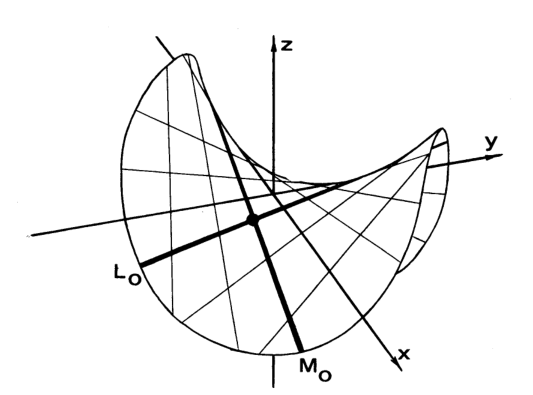
\includegraphics{Fig 02}
    \caption{The quadric surface in $\P^3$.}
    \label{fig1.2.4}
\end{figure}

\begin{proof}
    \begin{enumerate}[label = (\alph*)]
        \item This is defined by $\psi([a_0 : a_1], [b_0 : b_1]) = [a_0 b_0 : a_0 b_1 : a_1 b_0 : a_1 b_1]$. We had the map $k[z_{00}, z_{01}, z_{10}, z_{11}] \longrightarrow k[x_0, x_1, y_0, y_1]$ via $z_{ij} \mapsto x_i y_j$. By \ref{1.2.14} above, $\im \psi = Z(\ker \theta)$. Thus, we seek to show $\ker(\theta) = (z_{00} z_{11} - z_{01} z_{10})$.

        We will approach this with dimension theory. Note $z_{00} z_{11} - z_{01} z_{10}$ is irreducible and is in $\ker(\theta)$. Hence, $(z_{00} z_{11} - z_{01} z_{10}) \subseteq \ker(\theta)$ is an inclusion of primes, so we can prove equality by proving equality of their codimensions. By Krull's principal ideal theorem, the codimension of $(z_{00} z_{11} - z_{01} z_{10})$ is $1$. Furthermore, we have $\dim \im \theta = 4 - \codim \ker(\theta)$.

        We are therefore left to compute $\dim \im \theta$. Indeed, $\im \theta = k[x_0 y_0, x_0 y_1, x_1 y_0, x_1 y_1]$. To show that this has dimension $3$, we claim that the first three generators are independent and that the last is algebraic over the first three (really we could choose any $3$ of $4$). Indeed, the easy part is that $x_1 y_1$ satisfies $(x_0 y_0) t - (x_0 y_1)(x_1 y_0)$. Hence, $k(x_0 y_0, x_0 y_1, x_1 y_0, x_1 y_1) / k(x_0 y_0, x_0 y_1, x_1 y_0)$ is algebraic so their transcendence degrees agree.

        Now we want algebraic independence of these first $3$. Take indeed some $\sum a_{ijk} (x_0 y_0)^i (x_0 y_1)^j (x_1 y_0)^k = 0$. Then $\sum a_{ijk} x_0^{i+j} x_1^{k} y_0^{i + k} y_1^{j} = 0$. Observe that the map $(i, j k) \mapsto (i + j, k, i + k, j)$ is injective. Thus, each coefficient $a_{ijk}$ is attached to a monomial of a unique ``signature" $(i + j, k, i + k, j)$. $x_0, x_1, y_0, y_1$ are algebraically independent so these distinct signature monomials are linearly independent. Thus, each $a_{ijk} = 0$ and we have our algebraic independence.

        In conclusion, $\dim k[x_0 y_0, x_0 y_1, x_1 y_0, x_1 y_1] = 3$. Thus, $\ker(\theta)$ and $(z_{00} z_{11} - z_{10} z_{01})$ have the same codimension. Thus, they are equal and we conclude $\im \psi = Z(\ker \theta) = Z(z_{00} z_{11} - z_{01} z_{10})$.

        \item We have our map $\P^1 \times \P^1 \longrightarrow Q$. Fix some $t = [a : b] \in \P^1$. We'll define $L_t = \im(\psi(t, -))$ and $M_t = \im(\psi(-, t))$. This essentially transfers the coordinate grid on the plane onto quadric surface. As all these set theoretic properties hold for the coordinate grid in $\P^2$, the bijection $\psi$ proves that they hold in $Q$. We therefore need only show that these are in fact lines.

        Let $t = [a_0 : a_1]$. Then $L_t = \curly{[a_0 b_0 : a_0 b_1 : a_1 b_0 : a_1 b_1] : [b_0 : b_1] \in \P^1}$. We can observe that these satisfy the equations $a_1 z_{00} - a_0 z_{10}$ and $a_0 z_{11} - a_1 z_{01}$. Thus we easily have $L_t \subseteq Z(a_1 z_{00} - a_0 z_{10}) \cap Z(a_0 z_{11} - a_1 z_{01})$. On the other hand, suppose $[c_{00} : c_{01} : c_{10} : c_{11}]$ is in this line. Then if $a_0 \neq 0$ take $b_0 = c_{00}$ and $b_1 = c_{01}$. If $a_0 = 0$ take $b_0 = c_{10}$ and $b_1 = c_{11}$. One can check that the image of this in the Segre embedding along $t$ lies in $L_t$. We can do something analogous for $M_t$.

        \item $Q$ contains the image of the $2$-uple embedding $\P^1 \longrightarrow \P^3$, which has image $\curly{[a_0^2 : a_0 a_1 : a_1 a_0 : a_1^2]}$. See \ref{1.2.12} for why this is a curve. Note that it is also the image of the diagonal $\Delta \subseteq \P^1 \times \P^1$ under $\psi$. However, the diagonal is not closed as $\P^1$ is not Hausdorff. In fact, it is irreducible! This immediately shows that $\psi$ is not a homeomorphism, but for the sake of completeness, we will show that $\P^1 \times \P^1$ contains precisely the curves already described.

        First of all, let $L_t' = \curly{t} \times \P^1$ and $M_t' = \P^1 \times \curly{t}$, so that $\psi$ takes $L_t' \mapsto L_t$ and $M_t' \mapsto M_t$. We claim that these are the only curves in $\P^1 \times \P^1$. A curve is an irreducible closed subset of dimension $1$, which is a purely topological notion. To do this, we will first explore irreducible closed subsets of a product of spaces.

        \begin{lemma}
            Let $X_0, X_1$ be topological spaces. Then the irreducible closed subsets of $X_0 \times X_1$ are all of the form $A_0 \times A_1$ where $A_i \substeq X_i$ are irreducible closed subsets of their respective spaces.
        \end{lemma}
        \begin{proof}
            First, let's show that these proposed subsets are actually closed and irreducible. Closedness is immediate, so we focus on irreducibility. Take $\emptyset \neq U_0, U_1 \subseteq A_0 \times A_1$ open. Then we can find $U_{00} \times U_{01} \subseteq U_0$ and $U_{10} \times U_{11} \subseteq U_i$ open and nonempty. By irreducibilty of the $A_i$, $U_{i0} \cap U_{i1} \neq \emptyset$. Hence, $U_0 \cap U_1 \neq \emptyset$.

            Now, take $F \subseteq X_0 \times X_1$ irreducible and closed. Then we have $F \subseteq \pi_0[F] \times \pi_1[F]$, but these certainly need not be closed, so instead take $F \subseteq \overline{\pi_0[F]} \times \overline{\pi_1[F]} = Z$. Then $F$ is an irreducible closed subset of $Z$. As it is closed, $Z - F$ is open and disjoint from $F$. Assume that this is a proper containent and take therefore a basic open set $\emptyset \neq U_0 \times U_1 \subseteq Z - F$. Now, as $U_0 \times U_1 \subseteq Z - F$, $Z - (U_0 \times U_1) \supseteq F$. Furthermore, $Z - (U_0 \times U_1) \subseteq (X_0 - U_0) \times \overline{\pi_1[F]} \cup \overline{\pi_0[F]} \times (X_1 - U_1)$, which is closed. Then as $F$ is irreducible, it is contained in one of these, say $F \subseteq (X_0 - U_0) \times \overline{\pi_1[F]}$. In particular, $\pi_0[F] \subseteq X_0 - U_0$, so $\overline{\pi_0[F]} \subseteq X_0 - U_0$. But we took $U_0 \subseteq \overline{\pi_0[F]}$, a contradiction. Hence, $F = \overline{\pi_0[F]} \times \overline{\pi_1[F]}$. Why are these irreducible? Uhhhhhhhh cuz
        \end{proof}

        Note that the irreducible closed subsets of $\P^1$ are $\emptyset$, points, and the whole of $\P^1$. This therefore shows that the only curves in $\P^1$ are $L_t'$ and $M_t'$ as describe.
    \end{enumerate}
\end{proof}
